\begin{figure}[!htbp]
    % Row 1
    \def\subfigheight{4.5cm}
    \begin{subfigure}[t]{0.30\textwidth}
        %\includesvg[inkscapelatex=false,height=\subfigheight]{records/inverted/final_best_swim.svg}
        \includegraphics[height=\subfigheight]{final_best_swim_svg-raw.pdf}
        \caption{\texttt{SWIM} - \textbf{\swimrecord}\%}
    \end{subfigure}
    \hfill
    \begin{subfigure}[t]{0.45\textwidth}
        \centering
        %\includesvg[inkscapelatex=false,height=\subfigheight]{records/inverted/final_best_shirts.svg}
        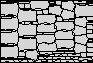
\includegraphics[height=\subfigheight]{final_best_shirts_svg-raw.pdf}
        \caption{\texttt{SHIRTS} - \textbf{\shirtsrecord}\%}
    \end{subfigure}
    \hfill
    \begin{subfigure}[t]{0.22\textwidth}
        \hfill
        %\includesvg[inkscapelatex=false,height=\subfigheight]{records/inverted/final_best_mao.svg}
        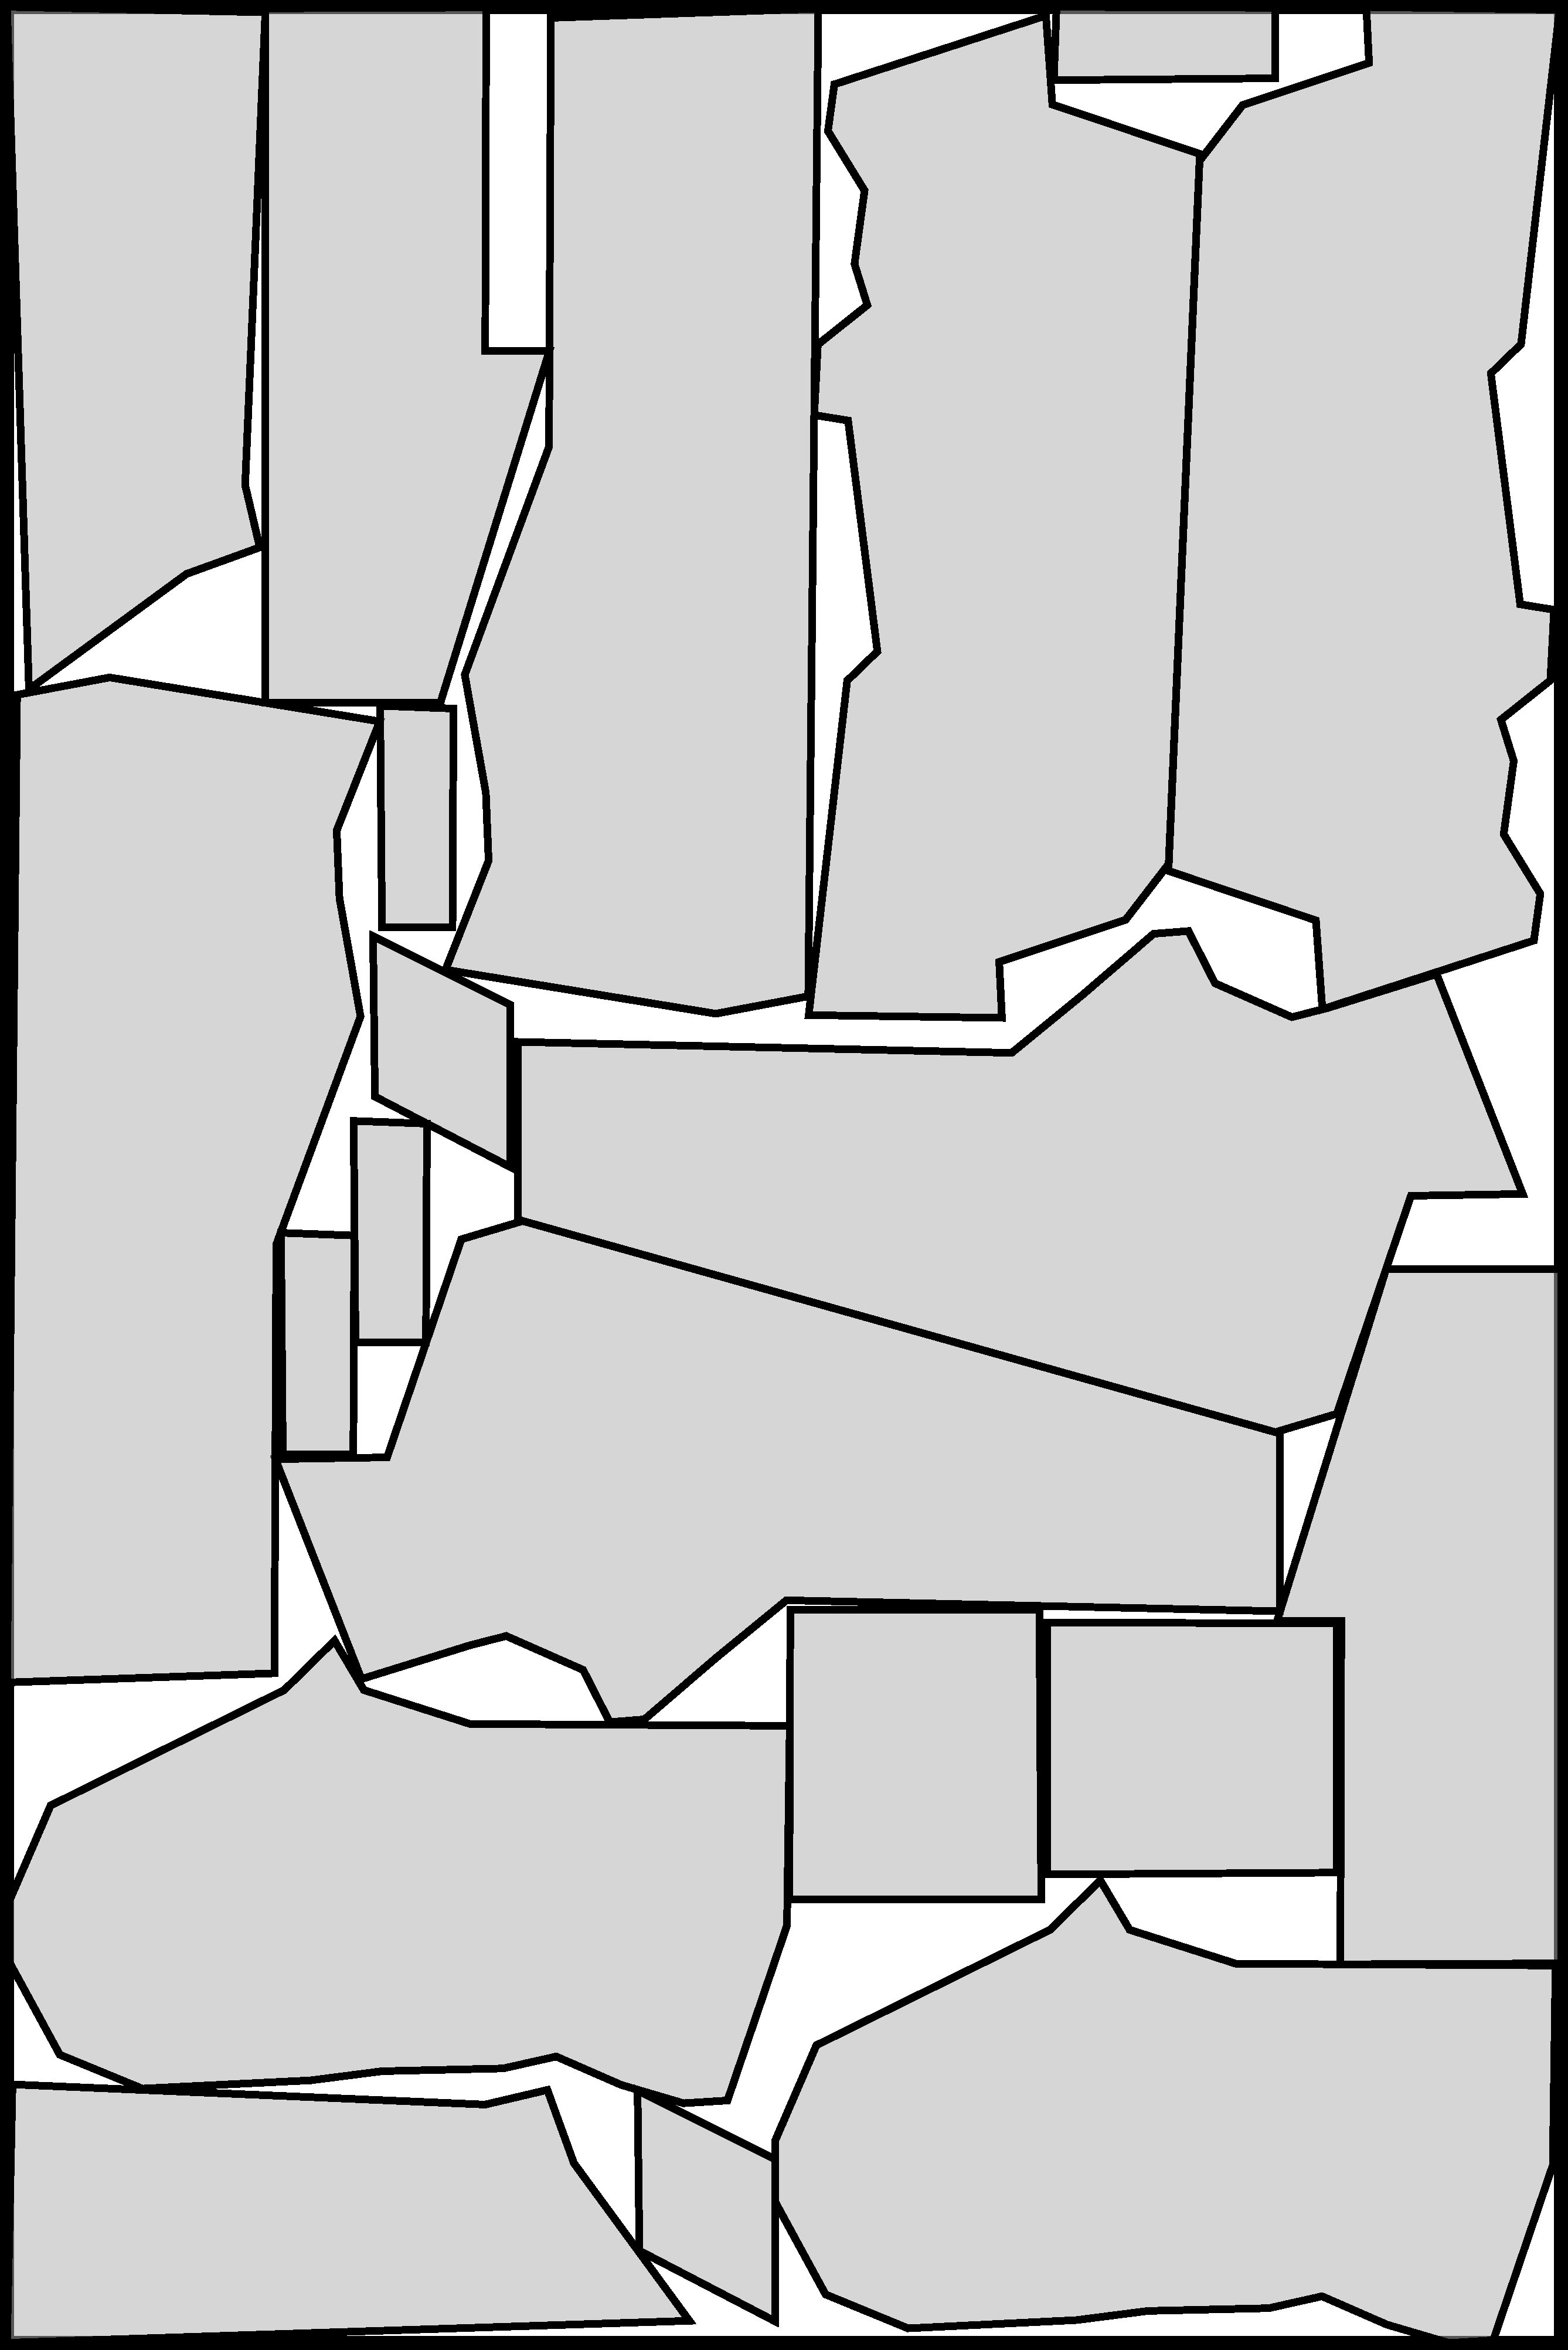
\includegraphics[height=\subfigheight]{final_best_mao_svg-raw.pdf}
        \caption{\texttt{MAO} - \textbf{86.87}\%}
    \end{subfigure}

    \vspace{.5em}
        
    % Row 2
    \def\subfigheight{3.2cm}
    \begin{subfigure}[t]{0.43\textwidth}
        %\includesvg[inkscapelatex=false,height=\subfigheight]{records/inverted/final_best_albano.svg}
        \includegraphics[height=\subfigheight]{final_best_albano_svg-raw.pdf}
        \caption{\texttt{ALBANO} - \textbf{89.82}\%}
    \end{subfigure}
    \hfill
    \begin{subfigure}[t]{0.36\textwidth}
        \centering
        %\includesvg[inkscapelatex=false,height=\subfigheight]{records/inverted/final_best_blaz1.svg}
        
\includegraphics[height=\subfigheight]{final_best_blaz1_svg-raw.pdf}
        \caption{\texttt{SHAPES2} - \textbf{86.23}\%}
    \end{subfigure}
    \hfill
    \begin{subfigure}[t]{0.16\textwidth}
        \hfill
        %\includesvg[inkscapelatex=false,height=\subfigheight]{records/inverted/final_best_marques.svg}
        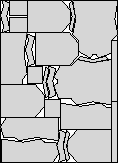
\includegraphics[height=\subfigheight]{final_best_marques_svg-raw.pdf}
        \caption{\texttt{MARQUES} \\ - \textbf{92.02}\%}
    \end{subfigure}
    
    \vspace{.5em}
    
    % Row 3
    \def\subfigheight{3.8cm}
    \begin{subfigure}[t]{0.76\linewidth}
        %\includesvg[inkscapelatex=false,height=\subfigheight]{records/inverted/final_best_trousers.svg}
        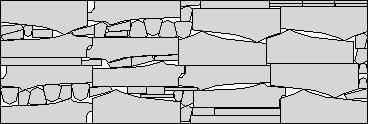
\includegraphics[height=\subfigheight]{final_best_trousers_svg-raw.pdf}
        \caption{\texttt{TROUSERS} - \textbf{\trousersrecord}\%}
    \end{subfigure}
    \hfill
    \begin{subfigure}[t]{0.11\linewidth}
        \centering %looks better
        %\includesvg[inkscapelatex=false,height=\subfigheight]{records/inverted/final_best_jakobs1.svg}
        
\includegraphics[height=\subfigheight]{final_best_jakobs1_svg-raw.pdf}
        \caption{\texttt{JAKOBS1}\\ - \textbf{\jakobsonerecord}\%}
    \end{subfigure}
    \hfill
    \begin{subfigure}[t]{0.10\linewidth}
        \hfill
        %\includesvg[inkscapelatex=false,height=\subfigheight]{records/inverted/final_best_jakobs2.svg}
        
\includegraphics[height=\subfigheight]{final_best_jakobs2_svg-raw.pdf}
        \caption{\texttt{JAKOBS2}\\ - 87.73\%}
    \end{subfigure}

    \vspace{.5em}

    % Row 4
    \def\subfigheight{3.1cm}
    \begin{subfigure}[t]{0.2\linewidth}
        %\includesvg[inkscapelatex=false,height=\subfigheight]{records/inverted/final_best_dagli.svg}
        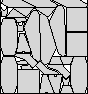
\includegraphics[height=\subfigheight]{final_best_dagli_svg-raw.pdf}
        \caption{\texttt{DAGLI} - \textbf{90.17}\%}
    \end{subfigure}
    \hfill
    \begin{subfigure}[t]{0.29\linewidth}
        \centering
        %\includesvg[inkscapelatex=false,height=\subfigheight]{records/inverted/final_best_shapes0.svg}
        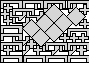
\includegraphics[height=\subfigheight]{final_best_shapes0_svg-raw.pdf}
        \caption{\texttt{SHAPES0} - \textbf{\shapeszerorecord}\%}
    \end{subfigure}
    \hfill
    \begin{subfigure}[t]{0.29\linewidth}
        \centering
        %\includesvg[inkscapelatex=false,height=\subfigheight]{records/inverted/final_best_shapes1.svg}
        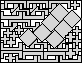
\includegraphics[height=\subfigheight]{final_best_shapes1_svg-raw.pdf}
        \caption{\texttt{SHAPES1} - 76.73\%}
    \end{subfigure}
    \hfill
    \begin{subfigure}[t]{0.17\linewidth}
        \hfill
        %\includesvg[inkscapelatex=false,height=\subfigheight]{records/inverted/final_best_fu.svg}
        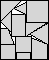
\includegraphics[height=\subfigheight]{final_best_fu_svg-raw.pdf}
        \caption{\texttt{FU} - 92.41\%}
    \end{subfigure}

    \caption{The best solutions obtained by \texttt{sparrow} (Table \ref{tab:best}) and their respective densities. Bold values indicate improved best-known solutions.}
    \label{fig:best_solutions}
\end{figure}